\subsection{Example 1}
The electrical system given in\cite{yang2025output} with parameters $C_t=2.2\mathrm{mF}$, $L_t=1.8\mathrm{mH}$ and $R_t=0.2\Omega$ is defined as the following state space model,
\begin{equation}
A=\begin{bmatrix}
    0& \frac{1}{C_t}\\
    -\frac{1}{L_t}& -\frac{-R_t}{L_t}    
\end{bmatrix},\,
B_w=\begin{bmatrix}
    -\frac{1}{C_t}\\
    0    
\end{bmatrix},\,
C=\begin{bmatrix}
    1& 0\\    
    1& 0\\    
    0& 1    
\end{bmatrix}
\end{equation}
where output redundancy is created by replicating the first output sensor as the second output sensor. The exogenous input matrix is chosen by combining the orthogonal component of output matrix with the output matrix as,
\begin{equation}
    D_w=C^\perp+C\begin{bmatrix}1\\1\end{bmatrix}=\begin{bmatrix}
    1.7071\\
    0.2929\\
    1.0000
    \end{bmatrix}
\end{equation}
A Luenberger observer is designed solving the LMI given in Eq~\ref{eq:lmi1} and is obtained as,
\begin{equation}
    L=\begin{bmatrix}
    -326.1332&  366.9908&   -5.2903\\
    -33.4833&   28.1920&   48.9023
    \end{bmatrix}
\end{equation}
noting that $B_w-LD_w=0$ is satisfied, hence the state estimation is not affected by the exogenous input. The estimated state can be used to obtain the exogenous input by utilizing,
\begin{equation}
    \hat{w}=D_w^\dagger(y-Cx)
\end{equation}
For the projection filtering the projection matrix given by Eq~\ref{eq:projection} is calculated for $C$ as,
\begin{equation}
\Pi^C=\begin{bmatrix}
    0.5&   -0.5&         0\\
    -0.5&    0.5&         0\\
    0&        0&         0
\end{bmatrix}
\end{equation}
where the projection for $D_w$ is,
\begin{equation}
\Pi^D_w=\begin{bmatrix}
    0.2714&   -0.1250&   -0.4268\\
   -0.1250&    0.9786&   -0.0732\\
   -0.4268&   -0.0732&    0.7500\\
\end{bmatrix}
\end{equation}
The state is filtered using,
\begin{equation}
    \hat{x}=(\Pi^D_w C)^\dagger (\Pi^D_w y)
\end{equation}
and the exogenous input is filtered using,
\begin{equation}
    \hat{w}=(\Pi^C D_w)^\dagger (\Pi^C y)
\end{equation}
The state estimation and the projection state filtering is compared in Figure~\ref{fig:ex1_states1}.
\begin{figure}[!htb]
    \centering
    
\includegraphics[width=0.85\linewidth]{img/ex1_states1}
    \caption{State filtering versus estimation of Example 1.}
    \label{fig:ex1_states1}
\end{figure}

The exogenous input estimated and filtered is depicted in Figure~\ref{fig:ex1_disturbance}.
\begin{figure}[!htb]
    \centering
    
\includegraphics[width=0.85\linewidth]{img/ex1_disturbance}
    \caption{Disturbance}
    \label{fig:ex1_disturbance}
\end{figure}

The projection filtering method utilizes the geometric properties of the output mapping, hence no dynamic estimation is present, it directly extracts the output map into its components. Despite the fact that the Luenberger observer gain for output redundant systems is able to eliminate the exogenous input term in the error dynamic by setting $B_w-LD_w$ to zero, the structure exploit performs better for the given example since no estimation takes place. Static output filtering fails if 
\begin{equation}
    D_w=C\alpha
\end{equation}
since,
\begin{equation}
    \Pi y=\Pi Cx+\Pi D_w w=\Pi C(x+\alpha)=0
\end{equation}
which shows that different channels need to exist in order separate signals using the projection. 

\subsection{Example 2}
Let the output mapping,
\begin{equation}
    y=Cx+D_ww+D_n n
\end{equation}
be given as,
\begin{equation}
    y=\begin{bmatrix}
    1&     0\\
    2&     1\\
    0&     1\\
    0&     1
    \end{bmatrix}x(t)+\begin{bmatrix}
        2.2060\\
        2.3970\\
        1.3015\\
        1.3015
    \end{bmatrix}w(t)+
    \begin{bmatrix}
    0.1960\\
    0.7382\\
    0.6697\\
    0.5265
    \end{bmatrix}n(t)
\end{equation}
where $w(t)$ is disturbance, $n(t)$ is noise and $x(t)$, which represents the system states, for illustrative purposes is chosen as,
\begin{equation}
    x(t)=\begin{bmatrix}
        \sin(t)\\ \cos(t)
    \end{bmatrix}
\end{equation}
The output mapping is modified as,
\begin{equation}
    y=Cx+\begin{bmatrix}
        D_w& D_n
    \end{bmatrix}\begin{bmatrix}
    w\\n        
    \end{bmatrix}
\end{equation}
and the projection is chosen as,
\begin{gather}
    \Pi^{wn}=I-\begin{bmatrix}
        D_w& D_n
    \end{bmatrix}\left(
        \begin{bmatrix}
        D_w\\ D_n
    \end{bmatrix}\begin{bmatrix}
        D_w& D_n
    \end{bmatrix}
    \right)\begin{bmatrix}
        D_w\\D_n
    \end{bmatrix}\\
    \Pi^{wn}=\begin{bmatrix}
    0.6224&   -0.2581&   -0.3034&   -0.2763\\
    -0.2581&    0.1118&    0.1698&    0.0618\\
    -0.3034&    0.1698&    0.5564&   -0.3549\\
    -0.2763&    0.0618&   -0.3549&    0.7094
    \end{bmatrix}
\end{gather}
The state $x(t)$ is recovered using,
\begin{gather}
    \hat{x}=(\Pi^{wn}C)^\dagger (\Pi^{wn}y)
\end{gather}

The output filtering results are depicted in Figure~\ref{fig:ex2_results}.
\begin{figure}[!htb]
    \centering
    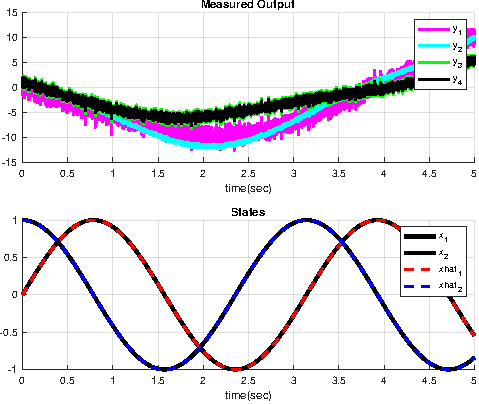
\includegraphics[width=0.85\linewidth]{img/ex2_results}
    \caption{State recovery}
    \label{fig:ex2_results}
\end{figure}

The disturbance is recovered using the projection,
\begin{gather}
    \Pi^{xn}=I-\begin{bmatrix}
        C& D_n
    \end{bmatrix}\left(
        \begin{bmatrix}
        C\\ D_n
    \end{bmatrix}\begin{bmatrix}
        C& D_n
    \end{bmatrix}
    \right)\begin{bmatrix}
        C\\D_n
    \end{bmatrix}\\
    \Pi^{xn}=\begin{bmatrix}
     0.7254&   -0.3627&    0.1507&    0.2120\\
   -0.3627 &   0.1813 &  -0.0754 &  -0.1060\\
    0.1507 &  -0.0754 &   0.0313 &   0.0440\\
    0.2120 &  -0.1060 &   0.0440 &   0.0619
    \end{bmatrix}
\end{gather}
as depicted in Figure~\ref{fig:ex2_results2}.
\begin{figure}[!htb]
    \centering
    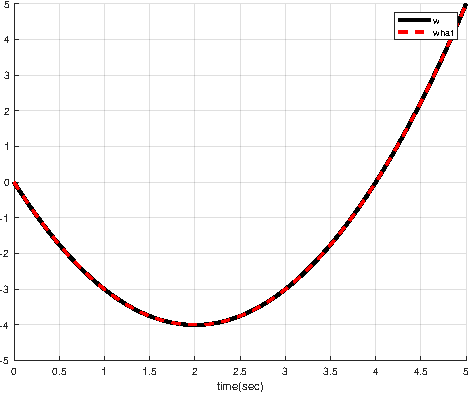
\includegraphics[width=0.85\linewidth]{img/ex2_results2}
    \caption{Disturbance recovery}
    \label{fig:ex2_results2}
\end{figure}
The state and disturbance recovery is successful as it can be observed from Figure~\ref{fig:ex2_results} and Figure~\ref{fig:ex2_results2}.

